\documentclass[../../thesis.tex]{subfiles}

\begin{document}

\section{Stage 1}

As mentioned in the section on representation learning, one needs to determine a set of tasks one wish to evaluate on, in order to say anything about the quality of the representations. We evaluate the representations based on two tasks

\subsection{Evaluation metrics}

\begin{itemize}
    \item \textbf{Reconstruction}: We evaluate the models ability to reconstruct the original data from latent representation. Success indicating perservation of information.
    \item \textbf{Downstream classification}: We evaluate the latent representations on its ability linear classification. 
    \item \textbf{Training time}
    \item \textbf{Number of parameters}
    \item 
\end{itemize}

\subsection{Reconstruction}

\subsection{Classification}

\subsection{Codebook investigations}

In the two tokenization models, how does the codebooks differ? Look at codebook utlization. Histograms across dimensions?  

\section{Stage 2}

\subsection{Evaluation metrics}
\begin{itemize}
    \item \textbf{IS}:
    \item \textbf{FID}:
    \item \textbf{Visual inspection}:
    \item \textbf{Token usage}:
    \item \textbf{Generating distribution}:
\end{itemize}


\section{Ablation studies}

\subsection{Augmentation Reconstruction Weight}

\begin{figure}[h]
    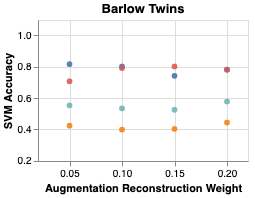
\includegraphics[scale=0.55]{BT_SVM_ReconsWeight.png}
    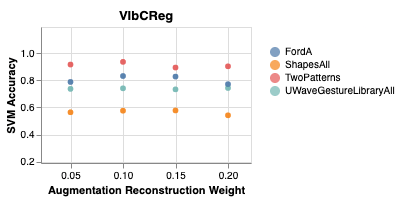
\includegraphics[scale=0.55]{ViB_SVM_ReconsWeight.png}
    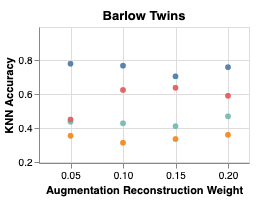
\includegraphics[scale=0.55]{BT_KNN_ReconsWeight.png}
    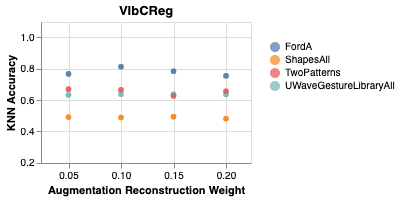
\includegraphics[scale=0.55]{ViB_KNN_ReconsWeight.png}
    \centering  
    \caption{Augmentations: Window Warp and amplitude resize. Averaged across 2 runs. Trained for 250 epochs}  
\end{figure}

\begin{figure}[h]
    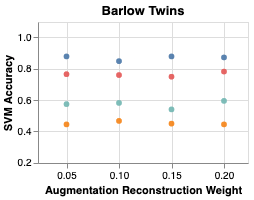
\includegraphics[scale=0.55]{BT_SVM_ReconsWeight_Slice.png}
    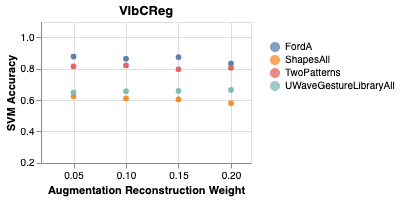
\includegraphics[scale=0.55]{ViB_SVM_ReconsWeight_Slice.png}
    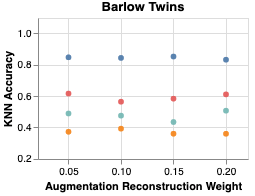
\includegraphics[scale=0.55]{BT_KNN_ReconsWeight_Slice.png}
    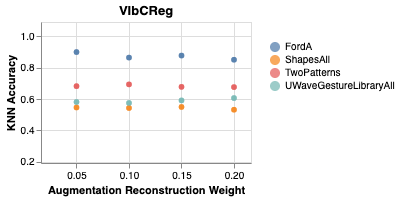
\includegraphics[scale=0.55]{ViB_KNN_ReconsWeight_Slice.png}

    % \centering  
    \caption{Augmentation: Slice and shuffle. Averaged across 2 runs. Trained for 250 epochs}  
\end{figure}

\begin{figure}[h]
    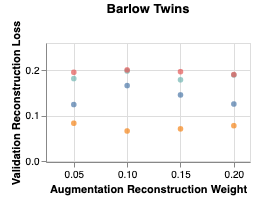
\includegraphics[scale=0.55]{BT_ValRecons_ReconsWeight.png}
    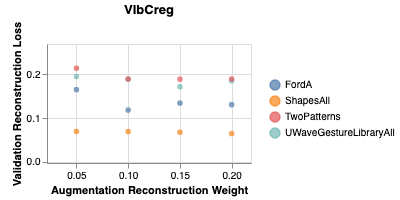
\includegraphics[scale=0.55]{ViB_ValRecons_ReconsWeight.png}
    % \centering  
    \caption{Augmentation: Slice and shuffle. Averaged across 2 runs. Trained for 250 epochs}  
\end{figure}
\begin{figure}[h]
    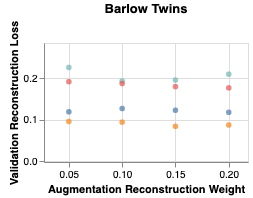
\includegraphics[scale=0.55]{BT_ValRecons_ReconsWeight_Slice.png}
    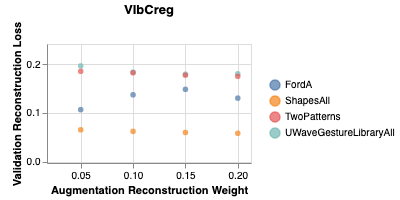
\includegraphics[scale=0.55]{ViB_ValRecons_ReconsWeight_Slice.png}
    % \centering  
    \caption{Augmentation: Slice and shuffle. Averaged across 2 runs. Trained for 250 epochs}  
\end{figure}
\subsection{Augmentation robustness}

\TODO{Download the Wandb data.}
Plot for each dataset and each augmentation: 
Mean KNN / SVM / ReconsLoss against augReconsWeight. 
Color code according to SSL-model.







\end{document}